\documentclass[11pt]{beamer}

\mode<presentation> {
\usetheme{Boadilla} }

\usepackage{graphicx} 
\usepackage{booktabs}
\usepackage[utf8]{inputenc}
\graphicspath{ {../../images/} }

\AtBeginSection[]{
  \begin{frame}
  \vfill
  \centering
  \begin{beamercolorbox}[sep=8pt,center,shadow=true,rounded=true]{title}
    \usebeamerfont{title}\insertsectionhead\par%
  \end{beamercolorbox}
  \vfill
  \end{frame}
}


%%%%%%%%%%%
%      Title Page      %
%%%%%%%%%%%
\title[Master Project]{Particle Filtering for Nonlinear State Space Models} 
\author[]{Hans-Peter H{\"o}llwirth \\ Supervisor: Christian Brownlees}
\institute[BGSE]{Barcelona Graduate School of Economics} 
\date{\today}

\begin{document}

\frame{\titlepage}

%%% Outline %%%
\begin{frame}
\frametitle{Outline}
\begin{itemize}
\item What I have done
\item State Space Models
\item Particle Filters
	\begin{itemize}
	\item Kalman Filter
	\item Sequential Importance Resampling (SIR)
	\item Continuous Sequential Importance Resampling (CSIR)
	\item Importance Sampling Particle Filter
	\end{itemize}
\item Evaluation
\item Illustration
	\begin{itemize}
	\item Trivariate Local Level Model
	\item Hierarchical Dynamic Poisson Model
	\end{itemize}
\end{itemize}
\end{frame}

%%%%%%%%%%%%%%%%
%      State Space Models      %
%%%%%%%%%%%%%%%%
\section{State Space Models}

%%% Local Level Model %%%
\begin{frame}
\frametitle{Local Level Model}
\begin{block}{Formulation}
\begin{center}
\begin{tabular}{ r r l }
  observation: & $y_t = x_t + \epsilon_t$, & $\epsilon_t \sim N(0,\sigma_{\epsilon}^2)$ \\
  state: & $x_{t+1} = x_t + \eta_t$, & $\eta_t \sim N(0,\sigma_{\eta}^2)$ \\
\end{tabular}
\end{center}
\end{block}
$$
\boldsymbol{\theta} = [\sigma_{\eta}^2,  \sigma_{\epsilon}^2]^T
$$
\begin{center}
\begin{tabular}{ r r l }
  transition density: & $x_{t+1} | x_t, \boldsymbol{\theta}$ & $\sim N(x_t,\sigma_{\epsilon}^2)$ \\
  measurement density: & $y_t | x_t, \boldsymbol{\theta}$ & $\sim N(x_t,\sigma_{\eta}^2)$ \\
\end{tabular}
\end{center}
\end{frame}

%%% Realization %%%
\begin{frame}
\frametitle{Local Level Realization}
\framesubtitle{$\sigma_{\eta}^2=1.4$, $\sigma_{\epsilon}^2=1.0$}

\centering
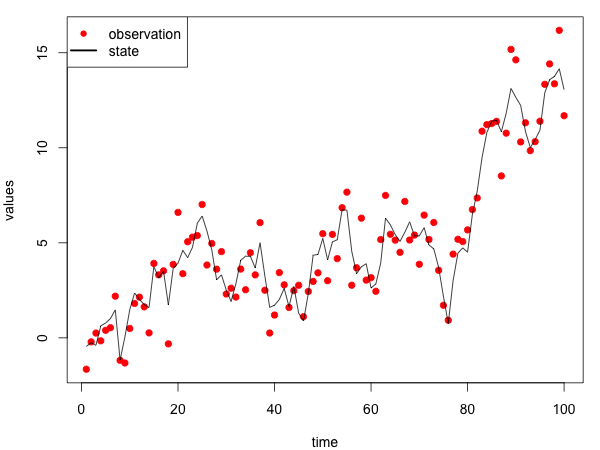
\includegraphics[scale=0.45]{ullm-realization}
\end{frame}

%%% Latent State Inference %%%
\begin{frame}
\frametitle{Latent State Inference}
\centering
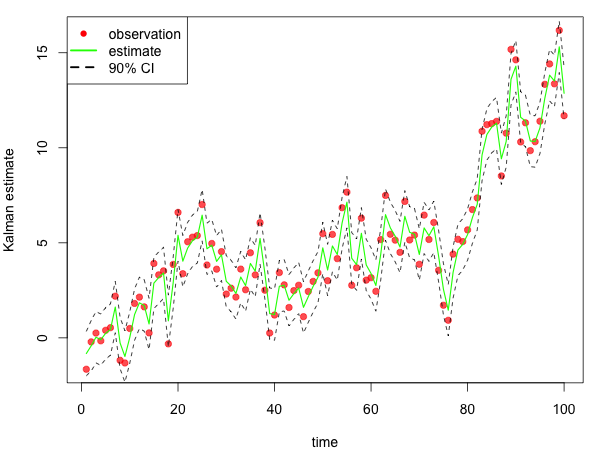
\includegraphics[scale=0.45]{ullm-estimate-kalman}
\end{frame}

%%% Parameter Inference %%%
\begin{frame}
\frametitle{Parameter Inference}
\centering
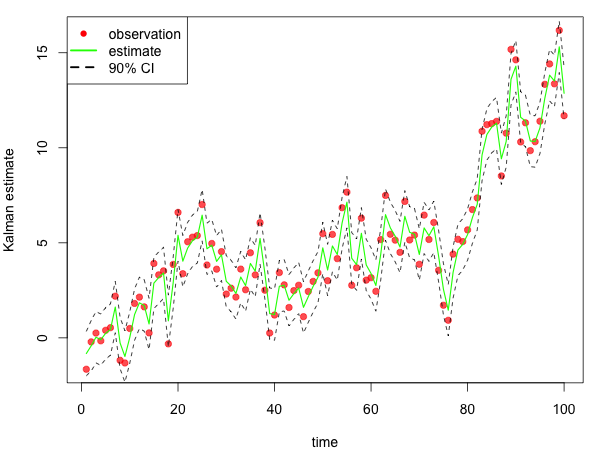
\includegraphics[scale=0.45]{ullm-estimate-kalman}
\end{frame}

%%%%%%%%%%%%%
%      Particle Filtering     %
%%%%%%%%%%%%%
\section{Particle Filtering}



%%%%%%%%%%%
%      Evaluation     %
%%%%%%%%%%%
\section{Evaluation}

%%% Method Comparison %%%
\begin{frame}
\frametitle{Method Comparison}
\centering
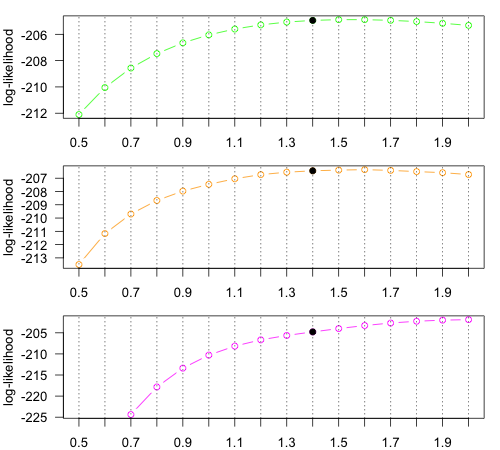
\includegraphics[scale=0.30]{ullm-loglik-eta}
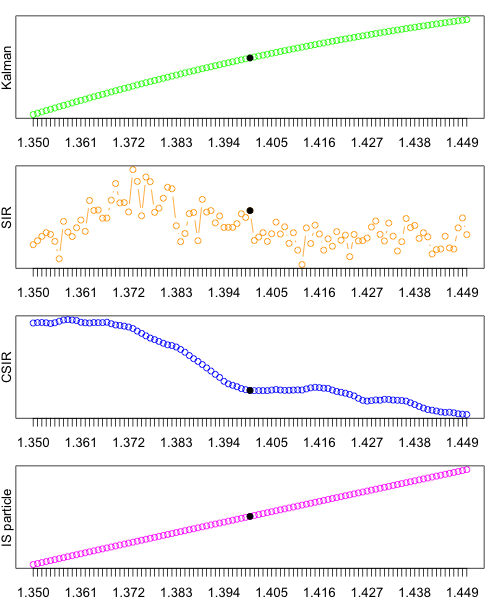
\includegraphics[scale=0.30]{ullm-loglik-zoom}
\end{frame}

%%% Method Comparison %%%
\begin{frame}
\frametitle{Method Comparison}
\begin{table}
\centering
\begin{tabular}{lccl}
\hline
Filter  & Latent state & Parameter & Comment\\
\hline
Kalman    & x & x & linear Gaussian models only\\
SIR      & x & &\\
CSIR      & x & x & univariate models only\\
IS      & & x & \\
\hline
\end{tabular}
\end{table}
\end{frame}

%%% Monte Carlo Simulations %%%
\begin{frame}
\frametitle{Monte Carlo Simulations}
\centering
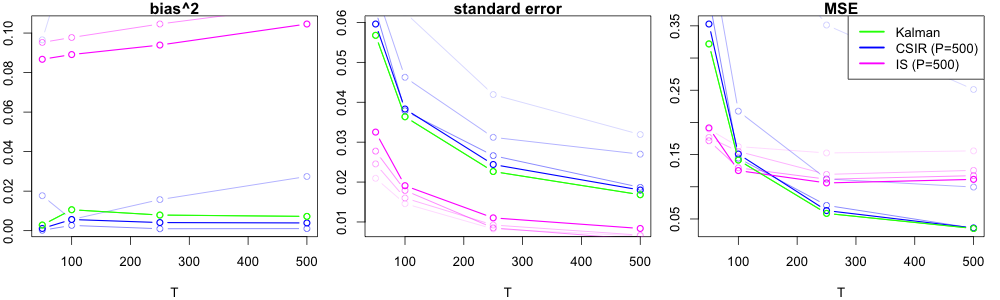
\includegraphics[scale=0.30]{ullm-mc-mle}
\end{frame}

%%%%%%%%%%
%      Illustration     %
%%%%%%%%%%
\section{Illustration}

%%% Trivariate Local Level Model %%%
\begin{frame}
\frametitle{Trivariate Local Level Model}
\begin{block}{Formulation}
\begin{center}
\begin{tabular}{ r r l }
  observation: & $\boldsymbol{y}_t = \boldsymbol{x}_t + \boldsymbol{\epsilon}_t$, & $\boldsymbol{\epsilon}_t \sim N(\textbf{0}, \sigma_{\epsilon}^2 I_3)$ \\
  state: & $\boldsymbol{x}_{t+1} = \boldsymbol{x}_t + \boldsymbol{\eta}_t$, & $\boldsymbol{\eta}_t \sim N(\textbf{0}, \Sigma_{\eta})$ \\
\end{tabular}
\end{center}
\end{block}
$$
\Sigma_{\eta} = 
\begin{bmatrix}
\sigma_{\eta 1}^2 & \rho \sigma_{\eta 1} \sigma_{\eta 2} & \rho \sigma_{\eta 1} \sigma_{\eta 3}
\\ \rho \sigma_{\eta 1} \sigma_{\eta 2} & \sigma_{\eta 2}^2 & \rho \sigma_{\eta 2} \sigma_{\eta 3}
\\ \rho \sigma_{\eta 1} \sigma_{\eta 3} & \rho \sigma_{\eta 2} \sigma_{\eta 3} & \sigma_{\eta 3}^2
\end{bmatrix}
$$
\bigskip
$$
\boldsymbol{\theta} = [\rho, \sigma_{\eta 1}^2, \sigma_{\eta 2}^2, \sigma_{\eta 3}^2, \sigma_{\epsilon}^2]^T
$$
\end{frame}

%%% Realization %%%
\begin{frame}
\frametitle{Trivariate Local Level Realization}
\centering
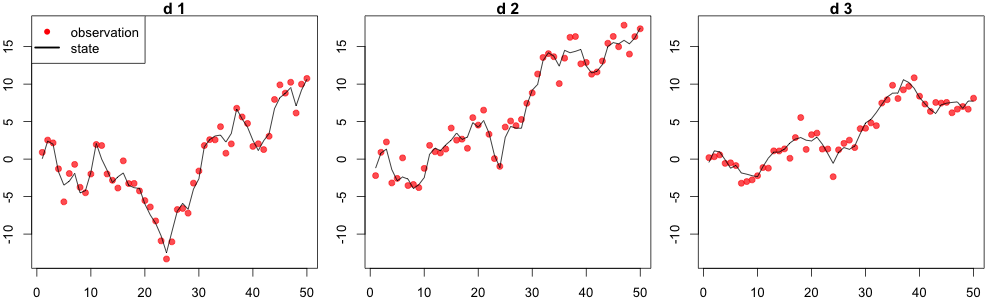
\includegraphics[scale=0.35]{mllm-realization-v2}\\
\bigskip
$\boldsymbol{\theta} = [\rho = 0.7, \sigma_{\eta 1}^2 = 4.2, \sigma_{\eta 2}^2 = 2.8, \sigma_{\eta 3}^2 = 0.9, \sigma_{\epsilon}^2 = 1.0]^T$
\end{frame}

%%% Latent State Inference %%%
\begin{frame}
\frametitle{Latent State Inference}
\framesubtitle{Kalman filter}
\centering
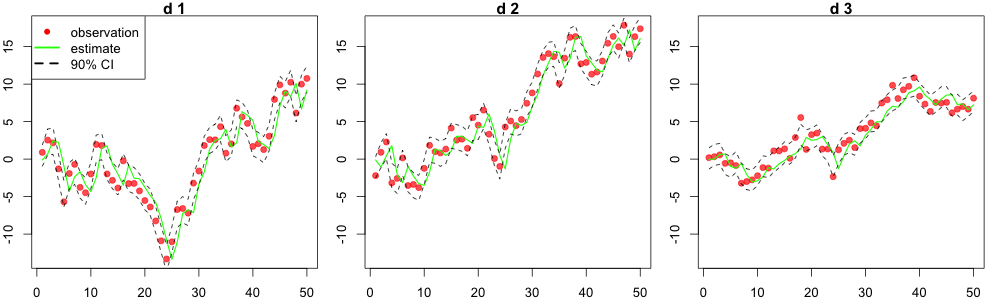
\includegraphics[scale=0.35]{mllm-estimate-kalman}
\end{frame}

\begin{frame}
\frametitle{Latent State Inference}
\framesubtitle{SIR particle filter}
\centering
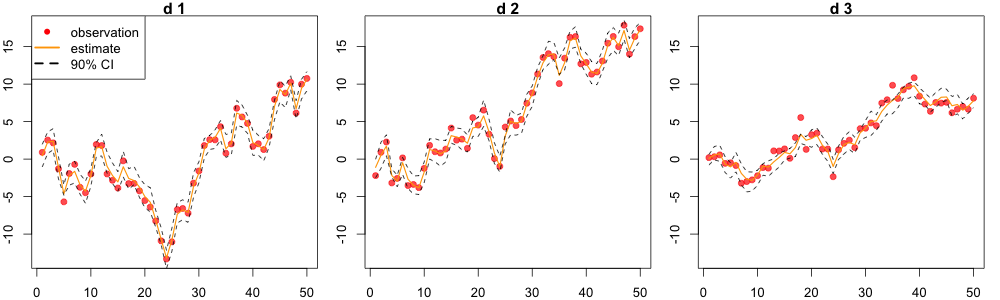
\includegraphics[scale=0.35]{mllm-estimate-sir}
\end{frame}

%%% Parameter Inference %%%
\begin{frame}
\frametitle{Parameter Inference}
\framesubtitle{Log-likelihood plots for $\sigma_{\eta 2}^2$ and $\rho$}
\centering
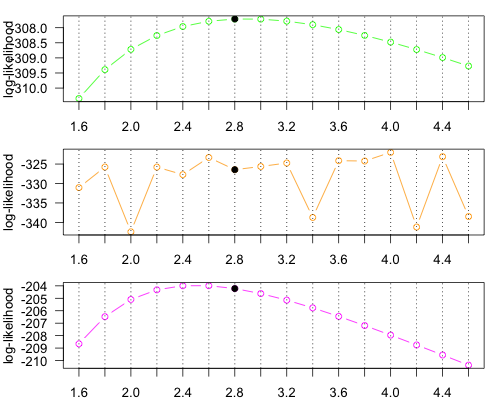
\includegraphics[scale=0.30]{mllm-loglik-var2}
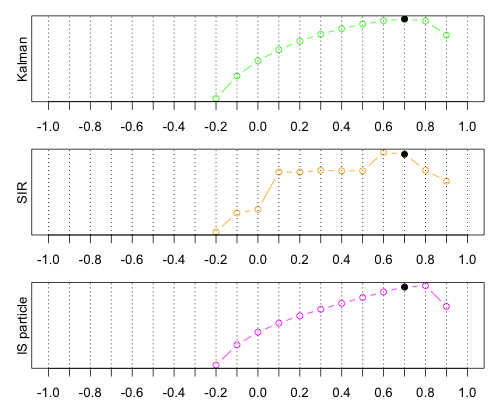
\includegraphics[scale=0.30]{mllm-loglik-rho}
\end{frame}

\begin{frame}
\frametitle{Parameter Inference}
\framesubtitle{Results}
\begin{table}
\centering
\begin{tabular}{l r r r r r r}
\hline
& $\sigma_{\eta 1}^2$ &  $\sigma_{\eta 2}^2$ & $\sigma_{\eta 3}^2$ & $\rho$ & true $\log \mathcal{L} $ & MLE $\log \mathcal{L} $ \\
\hline
True        & 4.20  & 2.80 &  0.90 & 0.70&  &  \\
Kalman   & 4.96  & 3.10  & 1.01 & 0.73 & -307.712 & -307.459 \\
SIR         & 2.27  & 1.53  & 1.29 & 0.52 & -313.466 & -336.291 \\
IS            & 2.69  & 2.09  & 1.06 & 0.42 &  & \\
\hline
\end{tabular}
\end{table}
\end{frame}

%%% Hierarchical Dynamic Poisson Model %%%
\begin{frame}
\frametitle{Hierarchical Dynamic Poisson Model}
\begin{block}{Formulation}
\begin{center}
\begin{tabular}{ r r l }
  observation: & $y_{m,n}$ & $\sim \text{Poisson}(\lambda_{m,n})$\\
  state: & $\log \lambda_{m,n}$ & $= \log \lambda_m^{(D)} + \log \lambda_{m,n}^{(I)} + \log \lambda_n^{(P)}$\\  
\end{tabular}
\end{center}
\end{block}
\begin{center}
\begin{tabular}{ r l l l}
  daily:& $\log \lambda_{m+1}^{(D)}$ &$= \phi_0^{(D)} + \phi_1^{(D)} \log \lambda_{m}^{(D)}  + \eta_m^{(D)}$ & $\eta_t \sim N(0, \sigma^2_{(D)})$ \\
  intra-daily:& $\log \lambda_{m,n+1}^{(I)}$ &$= \phi_1^{(I)} \log \lambda_{m,n}^{(I)}  + \eta_{m,n}^{(I)}$ & $\eta_{m,n} \sim N(0, \sigma^2_{(I)})$ \\
    periodic:& $\log \lambda_n^{(P)} $ &$= \phi_1^{(P)} \sin(\pi (n-1)/M)$ &\\
\end{tabular}
\end{center}
\bigskip
$$
\boldsymbol{\theta} = [ \phi_0^{(D)},  \phi_1^{(D)}, \sigma^2_{(D)}, \phi_1^{(I)}, \sigma^2_{(I)}, \phi_1^{(P)}]^T
$$
\end{frame}

%%% Realization %%%
\begin{frame}
\frametitle{Hierarchical Dynamic Poisson Realization}
\framesubtitle{$N=5$, $M=20$}
\centering
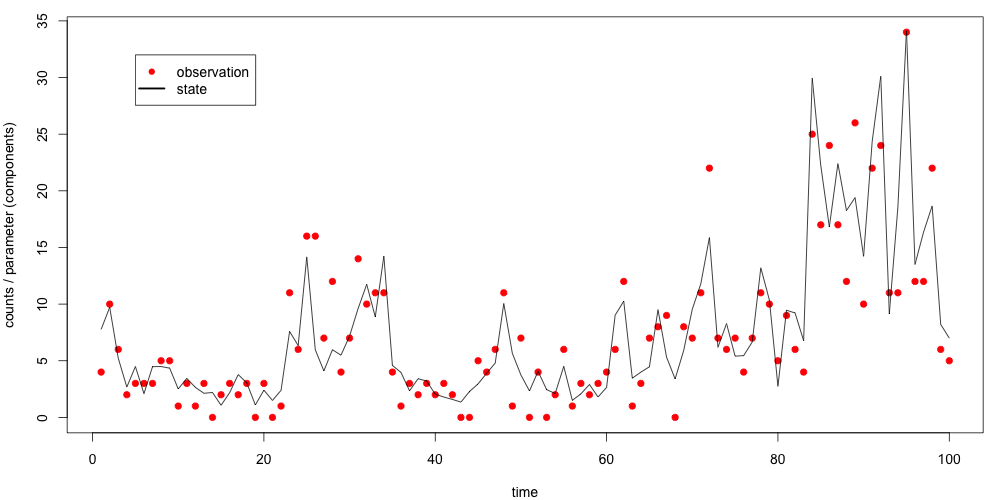
\includegraphics[scale=0.45]{hdpm-realization.png}\\
\bigskip
\small
$\boldsymbol{\theta} = [ \phi_0^{(D)} = 0.7,  \phi_1^{(D)} = 0.6, \sigma^2_{(D)} = 0.6, \phi_1^{(I)} = 0.3, \sigma^2_{(I)} = 0.2, \phi_1^{(P)} = 0.8]^T$
\par
\end{frame}

\begin{frame}
\frametitle{Hierarchical Dynamic Poisson Realization}
\framesubtitle{Components}
\centering
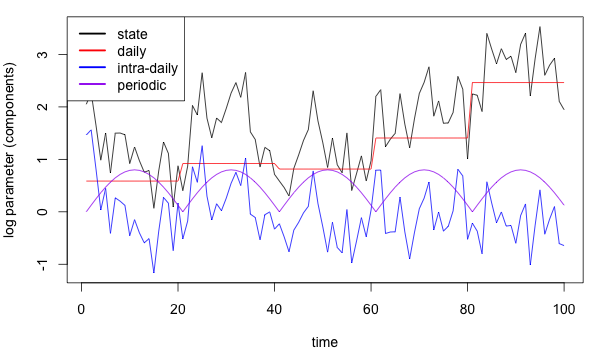
\includegraphics[scale=0.45]{hdpm-log-param}\\
\bigskip
\small
$\boldsymbol{\theta} = [ \phi_0^{(D)} = 0.7,  \phi_1^{(D)} = 0.6, \sigma^2_{(D)} = 0.6, \phi_1^{(I)} = 0.3, \sigma^2_{(I)} = 0.2, \phi_1^{(P)} = 0.8]^T$
\par
\end{frame}

%%% Latent State Inference %%%
\begin{frame}
\frametitle{Latent State Inference}
\framesubtitle{SIR particle filter}
\centering
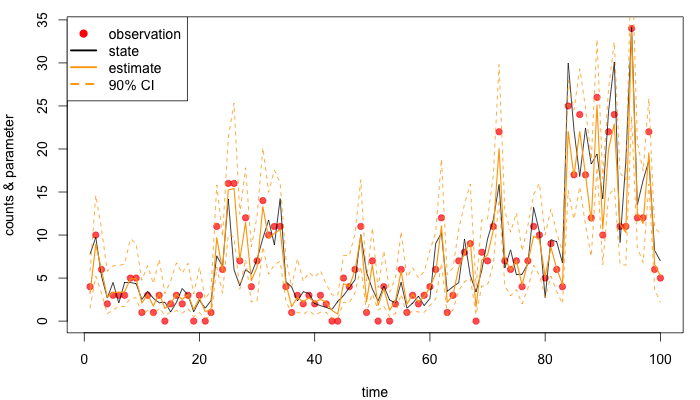
\includegraphics[scale=0.45]{hdpm-est}
\end{frame}

%%% Parameter Inference %%%
\begin{frame}
\frametitle{Parameter Inference}
\framesubtitle{Log-likelihood plots for $\phi_1^{(D)}$}
\centering
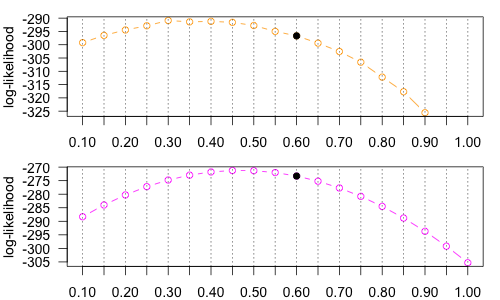
\includegraphics[scale=0.30]{hdpm-loglik-Dphi1}
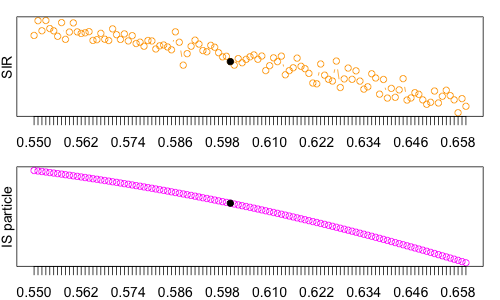
\includegraphics[scale=0.30]{hdpm-loglik-Dphi1-zoom}
\end{frame}

\begin{frame}
\frametitle{Parameter Inference}
\framesubtitle{Log-likelihood plots for $\sigma_{(D)}^2$}
\centering
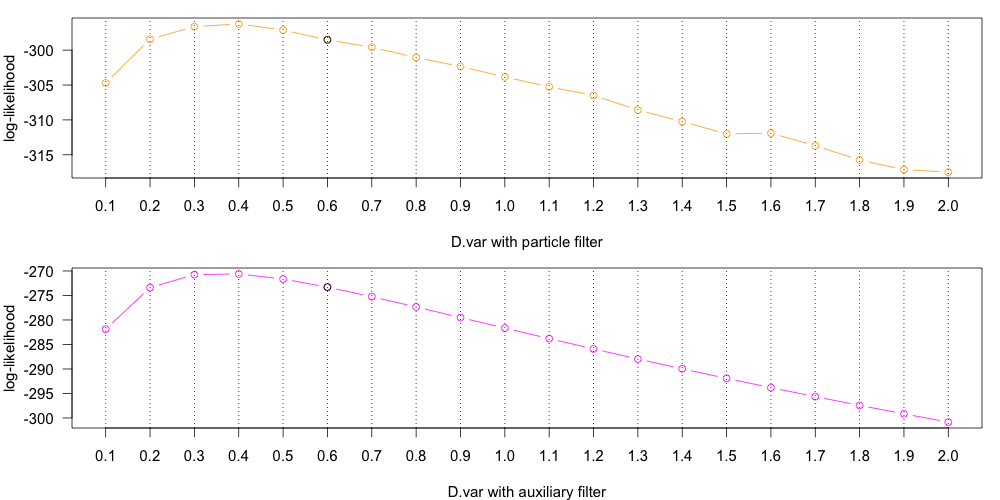
\includegraphics[scale=0.30]{hdpm-loglik-Dvar}
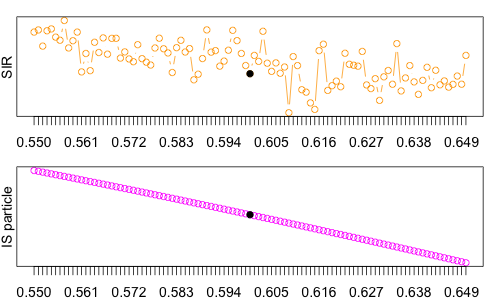
\includegraphics[scale=0.30]{hdpm-loglik-Dvar-zoom}
\end{frame}

\begin{frame}
\frametitle{Parameter Inference}
\framesubtitle{Results}
\begin{table}
\centering
\begin{tabular}{l r r r r r r}
\hline
& $\phi_0^{(D)}$ &  $\phi_1^{(D)}$ & $\sigma^2_{(D)}$ & $\phi_1^{(I)}$ & $\sigma^2_{(I)}$ & $\phi_1^{(P)}$\\
\hline
True        & 0.70  & 0.60 &  0.30 & 0.80 & 0.60 & 0.20\\
SIR         & 0.76  & 0.56  & 0.85 & 0.48 & 0.83 & 1.13\\
IS            & 0.65  & 0.59  & 0.40 & 0.63 & 0.35 & 0.31\\
\hline
\end{tabular}
\end{table}
\end{frame}

%%%%%%%
%      QA     %
%%%%%%%
\section{Q \& A}

\end{document}